% Q5V3: IoT sensor through wet earth — Signal path diagram
% Buried sensor → soil → air → gateway
\documentclass[border=10pt]{standalone}
\usepackage{tikz}
\usepackage{amsmath}
\usetikzlibrary{arrows.meta, decorations.pathreplacing}
\renewcommand{\familydefault}{\sfdefault}

\begin{document}
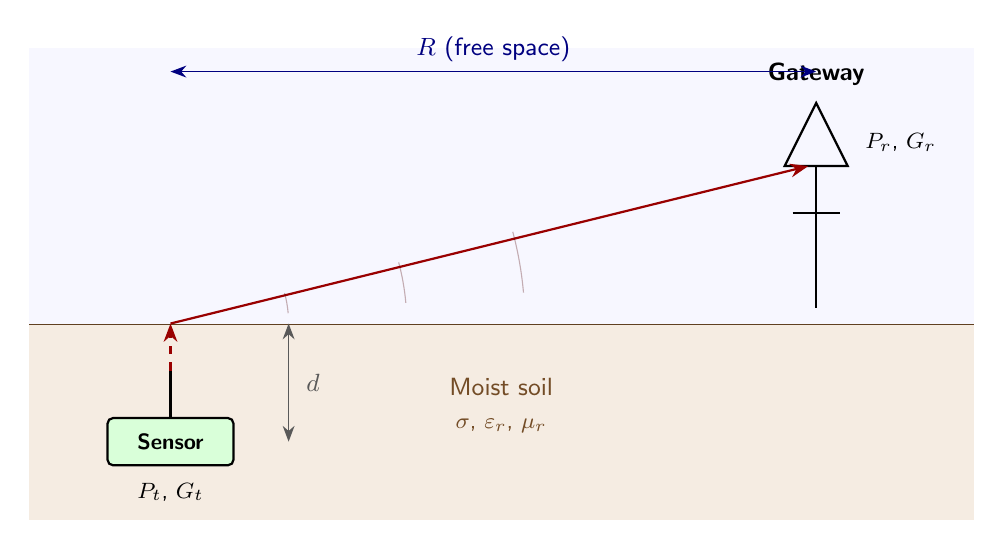
\begin{tikzpicture}[
    every node/.style={font=\sffamily},
    >=Stealth,
]

% === Ground ===
\fill[brown!15] (0,-2.5) rectangle (12,0);
\draw[thick, brown!50!black] (0,0) -- (12,0);
\node[above right, font=\sffamily\footnotesize, brown!50!black] at (0,0.05) {Ground surface};

% === Air region ===
\fill[blue!3] (0,0) rectangle (12,3.5);

% === Buried IoT sensor (Tx) ===
\draw[thick, rounded corners=2pt, fill=green!15] (1.0,-1.8) rectangle (2.6,-1.2);
\node[font=\sffamily\footnotesize\bfseries] at (1.8, -1.5) {Sensor};
\node[below, font=\sffamily\footnotesize] at (1.8, -1.9) {$P_t$, $G_t$};
% Antenna stub
\draw[thick] (1.8, -1.2) -- (1.8, -0.6);

% === Gateway receiver (Rx, far away) ===
% Tower icon
\draw[thick] (10, 0.2) -- (10, 2.0);
\draw[thick] (9.6, 2.0) -- (10, 2.8) -- (10.4, 2.0) -- cycle;
\draw[thick] (9.7, 1.4) -- (10.3, 1.4);
\node[above, font=\sffamily\small\bfseries] at (10, 2.9) {Gateway};
\node[right, font=\sffamily\footnotesize] at (10.5, 2.3) {$P_r$, $G_r$};

% === Signal path ===
% Through soil (upward)
\draw[->, thick, red!60!black, dashed] (1.8, -0.6) -- (1.8, 0);
% Through air (to gateway)
\draw[->, thick, red!60!black] (1.8, 0) -- (9.9, 2.0);

% Wave fronts in air
\foreach \r in {1.5, 3.0, 4.5} {
    \draw[thin, red!30!black, opacity=0.3]
        ({1.8+\r*cos(15)},{0+\r*sin(15)}) arc (15:5:\r);
}

% === Soil depth dimension ===
\draw[<->, line width=0.6pt, gray!70!black] (3.3, 0) -- (3.3, -1.5);
\node[right, font=\sffamily\small, gray!70!black] at (3.4, -0.75) {$d$};

% === Free-space distance ===
\draw[<->, line width=0.6pt, blue!50!black] (1.8, 3.2) -- (10, 3.2);
\node[above, font=\sffamily\small, blue!50!black] at (5.9, 3.2) {$R$ (free space)};

% === Soil labels ===
\node[font=\sffamily\small, brown!60!black] at (6, -0.8) {Moist soil};
\node[font=\sffamily\footnotesize, brown!60!black] at (6, -1.3) {$\sigma$, $\varepsilon_r$, $\mu_r$};

\end{tikzpicture}
\end{document}
